\subsection{Cavity measurements}\label{sec:cavity_measurements}

The cavity measurements here, primarily, outlined will be that of the double Fano cavity. The single Fano cavity measurement procedure will secondarily be clear as a simplification of the one for the double Fano cavity. 

Very simply put for the cavity measurement procedure, is that one must go through the Fano mirror alignment process outlined in section \ref{sec:grating_characterization} twice. One time for the bottom of the cavity, and then once for the top of the cavity, whereafter the two Fano mirrors are broad together according to the wanted cavity length and the transmission is recorded. However, this procedure contains many degrees of freedom and practicalities making it difficult to simply align each Fano mirror independently of each other. This section will go through each step of the process of arriving at a meaningful measurement of the transmission of the double Fano cavity. The reflections of improving the used method with be included in the discussion section.

%% Include reference to the discussion section when this is written.

\subsubsection{Aligning the double Fano cavity}

Before considering beginning to align the double Fano cavity, it is imperative to have two Fano mirrors which have similar physical dimensions, and thus be described by similar parameters as presented in section \ref{sec:fano_mirror}. In order to find a \emph{match}, the only valid method is to use brute force and simply characterize Fano mirrors until a match is found. The batch of tested Fano mirrors in this project all came from the same order delivered by Norcada, as this was assumed to provide the best chances for a match. The condition for the spectral detuning $\Delta = |\lambda_{0,1} - \lambda^{\prime}_{0,1}|$ of otherwise identical and lossless Fano mirrors is outlined in section \ref{sec:spectral_detuning}.

%% Appendix entry with all recorded spectra (all M gratings).

Assuming a match is found, which we denote $G_1$ and $G_2$\footnote{$G$ here stands for \emph{grating} while $1,2$ is indicative of the destinction between the two arbitrary Fano mirrors.}, the alingment process is given as follows: 
\begin{enumerate}
    \item The bottom, i.e. the arbitrary Fano mirror $G_1$, of the cavity is aligned according to the procedure outlined in section \ref{sec:grating_characterization}. This means that the incident beam is centered on and normal\footnote{A trick to determine the degree of accuracy of the angular alignment is to periodically block the light reflected from the Fano mirror, and thus make this flicker. This way the flickering light is easily distinguishable from the incoming light and by examining the light at apertures $I_2$ and $I_1$ from all sides perpendicular to the propagation direction, the needed angular adjustments become clear.} to $G_1$, and the polarization of the light is aligned such that the electric field is perpendicular to the grating lines. The wavelength of the laser is scanned, and the one corresponding to the guided-mode resonance of $G_1$ is recorded.  
    \item The bottom grating position is marked and the macor membrane holder (the macor membrane holder can be seen in figure \ref{fig:setup_zoomed}) containing $G_1$ is removed and stored safely. Now the laser polarization and spacial coordinates of $G_1$ are fixed and must not be changed in the following steps of the alignment procedure. The marks used to indicate the position of $G_1$ is shown in figure \ref{fig:bottom_with_alignment_mark}.
    \item The top part of the cavity is inserted, but \emph{without} the other Fano mirror $G_2$ in place, as the kinetic mirror- and rotational mounts first need to be centered in the beam. This is done by inserting a $100 \mu m$ pinhole, specifically designed for the purpose, into the rotational mount. The spacial and angular coordinates of the top mount is thus changed to maximize the signal through the pinhole. The centering is then tested by rotating the pinhole and ensuring that the signal does not change, i.e. that the center of the rotational mount does not move out of the beam by rotating it. When this is satisfied, the top mount is removed and the spacial coordinates are considered aligned and thus fixed. The so-called \emph{pinhole alignment method} will be explaied in greater detail in section \ref{sec:pinhole_method}.
    \item The Fano mirror $G_2$ is placed, with tape, onto the xy-adjustable mount (see figure \ref{fig:setup_zoomed}), which is then fastened to the rotational mount. The top mount now completely resembles the one shown in figure \ref{fig:cavity_setup_top_separate_pic}. $G_2$ is now aligned following a similar structure as the one outlined in section \ref{sec:grating_characterization}, but with the contraint of the above parameters being fixed. $G_2$ is moved into a position where it is centered with respect to the incident beam by adjusting the xy-adjustable mount, and the Fano mirror itself is now rotated to match the polarization of the laser. The angular alignment is done very similarly to that of $G_1$, as the kinetic mirror mount is here used. When $G_2$ is aligned, the wavelength is once again scanned, and the one matching the guided-mode of $G_2$ is recorded.
    \item The top mount, including $G_2$, is now removed from the setup and all degrees of freedom are expected to be aligned. The trick to make sure that the angular alignment is preserved when re-inserting the top mount is that the back reflection is centered in the aperture $I_4$ depicted in figure \ref{fig:setup_sketch}, this way one can quite easily regain the approximate angular alignment.
    \item The macor mebrane holder, with $G_1$ placed on it, is now re-inserted into the bottom of the setup and the Toptica laser is set to the guided-mode resonance wavelength according to $G_1$. In this way $G_1$ is carefully placed according to the marked position (see figure \ref{fig:bottom_with_alignment_mark}) and adjusted, by hand, to achieve the same minimum transmission as before it was removed. 
    \item The top mount, including $G_2$, is now too re-inserted, and adjusted by hand such that the back-reflected beam overlaps with the aperture $I_4$. 
    \item The wavelength of the Toptica laser is now set to the transmission wavelength given in eq. (\ref{eq:transmission_wavelength}), the wavelength exactly between the guided-mode resonance wavelengths of $G_1$ and $G_2$, i.e. $\lambda_t = (\lambda_{0,G_1} + \lambda_{0,G_2})/2$. 
\end{enumerate}

\begin{figure}[h!]
    \centering
    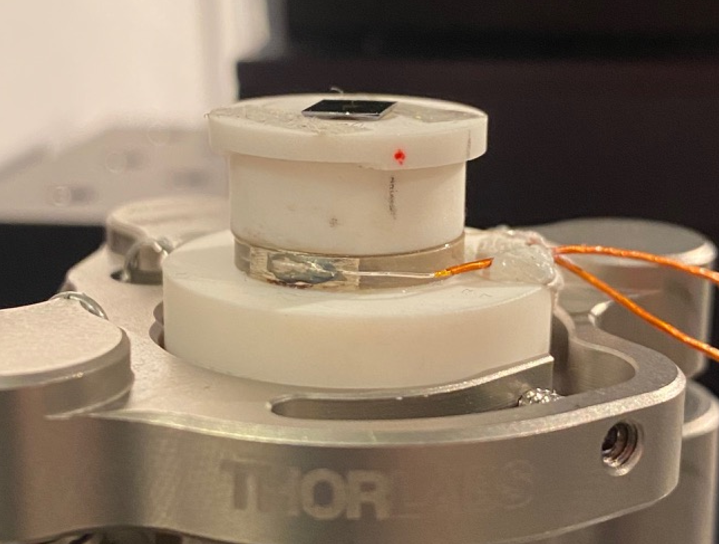
\includegraphics[width=0.5\textwidth]{figures/bottom_with_alignement_mark.pdf}
    \caption{A close-up of the bottom part of the cavity with a Fano mirror placed on the macor membrane holder. Note the marks used to re-insert the bottom part of the cavity as mentioned in steps 2 and 6.}
    \label{fig:bottom_with_alignment_mark}
\end{figure}

\subsubsection{Cavity resonance - the piezo ring}

Once the double Fano cavity is succesfully aligned with respect to the individual guided-modes of $G_1$ and $G_2$, the cavity mode (i.e. the cavity length) must be made to coincide in order to excite the Fano resonance mode. Here we remember that the cavity length is related to the cavity mode through the general Fabry-Perot cavity brightness condition $2 l = m \lambda$. 

In order to tune the cavity length on the scale necessary, it is scanned by periodically varying the length of the cavity using the piezo ring and applying an alternating current specified with the frequency generator shown in figure \ref{fig:freq_generator}. In this way the resulting signal recorded with photo detector $P_T$ and seen in the oscilloscope shown in figure \ref{fig:scope} is time-dependent and seen as fringes. Figure \ref{fig:length_scan} shows the corresponding fringes for an approximate cavity length of $100 \mu m$, both simulated and as data obtained directly from the oscilloscope screen.

\begin{figure}[h!]
    \centering
    \begin{subfigure}[b]{0.49\textwidth}
        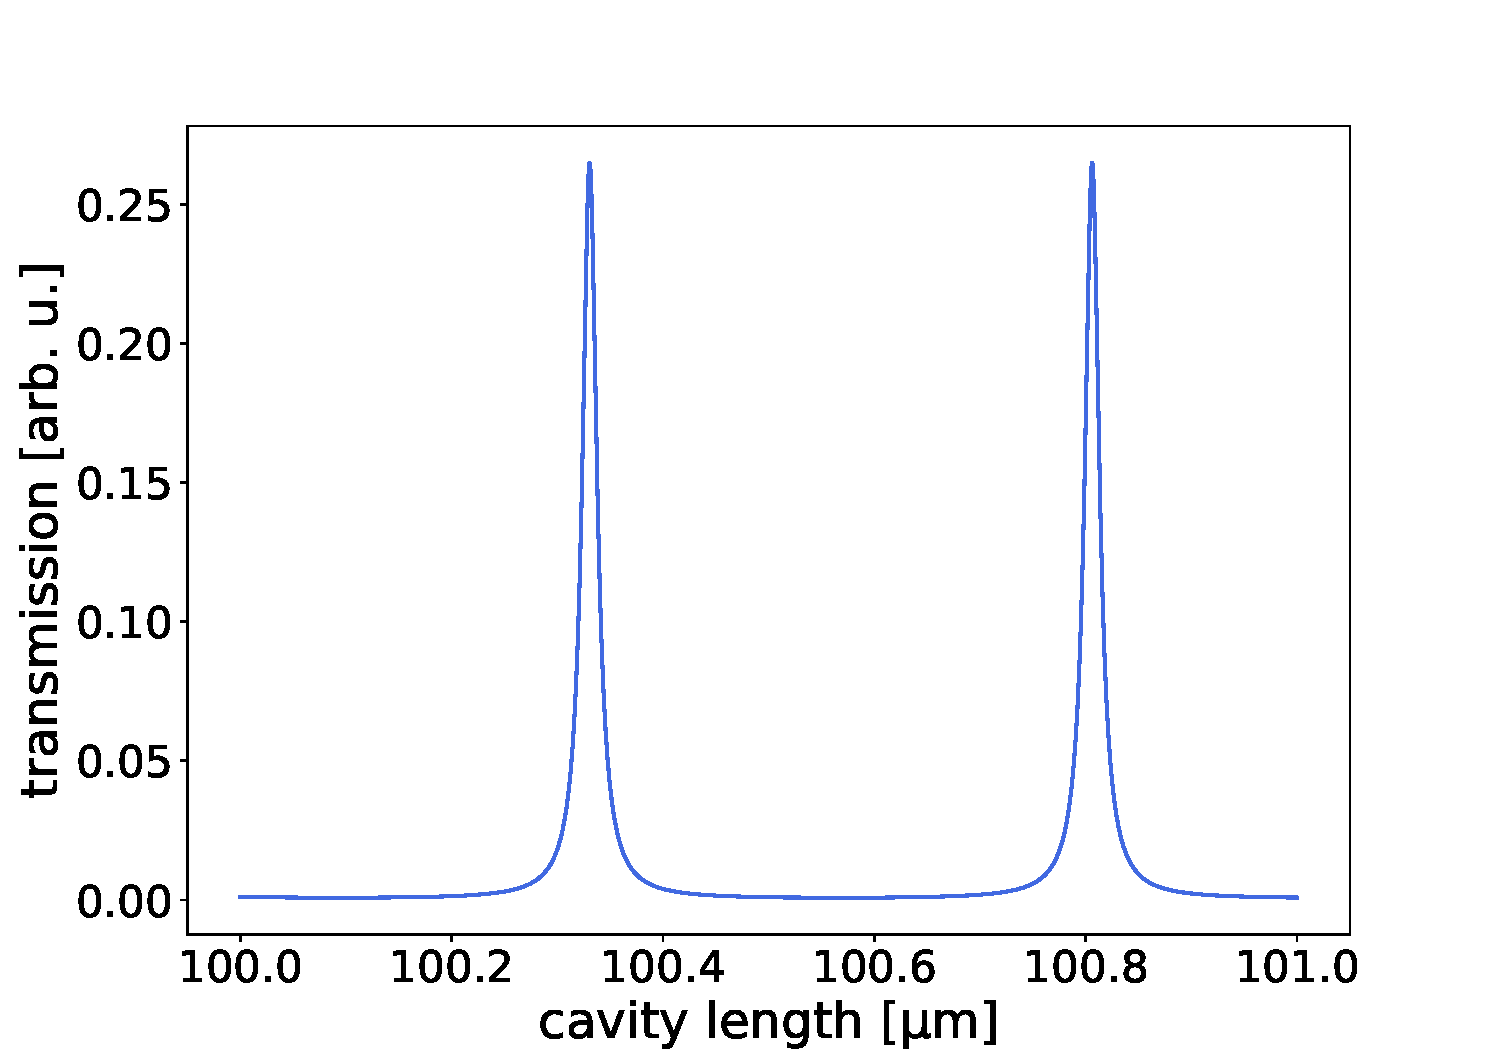
\includegraphics[width=\textwidth]{figures/length_scan_symmetric_lossless.pdf}
        \caption{}
        \label{fig:length_scan_sim}
    \end{subfigure}
    \begin{subfigure}[b]{0.49\textwidth}
        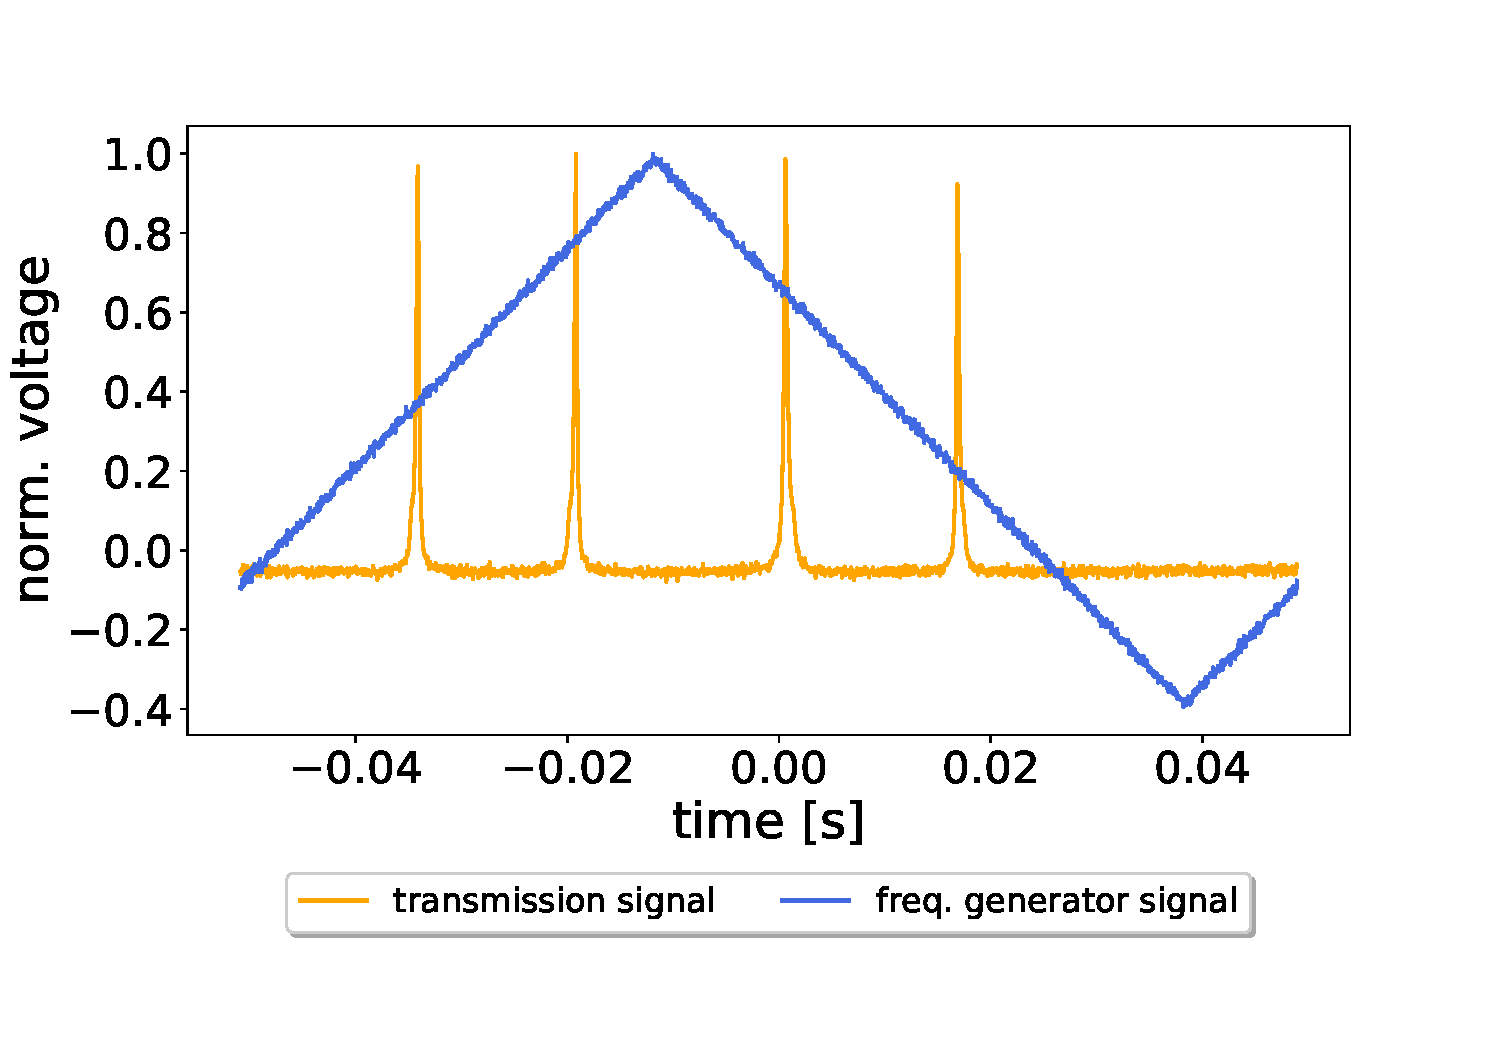
\includegraphics[width=\textwidth]{figures/scope_screenshot.pdf}
        \caption{}
        \label{fig:lenght_scan_scope}
    \end{subfigure}
    \caption{(a) shows a simulated length scan  of range $1 \mu m$ for a symmetric lossless double Fano cavity of length $\sim 100 \mu m$. The labeled resonant length $l_{res}$ in the figure indicates the first length found that fulfills the brightness condition. (b) is a plot of raw data logged from the oscilloscope used to record cavity transmission data. The blue line shows the signal from a frequency generator which is applied to the piezo ring, i.e. it correlates to the piezo expansion and thus a change in the cavity length. The orange line represents normalized cavity transmission intensity as a function of time, i.e. the cavity length. Note that the triangular signal is necesarry in order to uniformly expand and compress the piezo ring. This ensures that the FSR stems from a linear expansion and that the piezo ring does not break from non-linear stress across the crystal structure.}
    \label{fig:length_scan}
\end{figure}

When the fringes on the time-dependent length scan are visible while scanning with the piezo ring, they can be optimized by making small adjustments of the angular degrees of freedom of the top of the cavity, i.e. of $G_2$. The parallelisme of the cavity is an important parameter for a cavity of high finesse, and while normal incidence have here been achieved for $G_1$ and $G_2$ individually, both Fano mirrors have since been removed and re-inserted into the setup, which introduces uncertainty regarding the fine-tuning of the alignment. Especially the top of the cavity, which is fastened on nothing more than an optical post from Thorlabs and thus have only approximate reproducability of the angular alignment (this is seen in figure \ref{fig:cavity_setup_top_separate_pic}), is prone to uncertainties hereof after re-insertion. For this reason the parallelism is optimized using the fringes on the oscilloscope. The parallelism is outlined in greater detail in section \ref{sec:parallelism}.

\begin{figure}[h!]
    \centering
    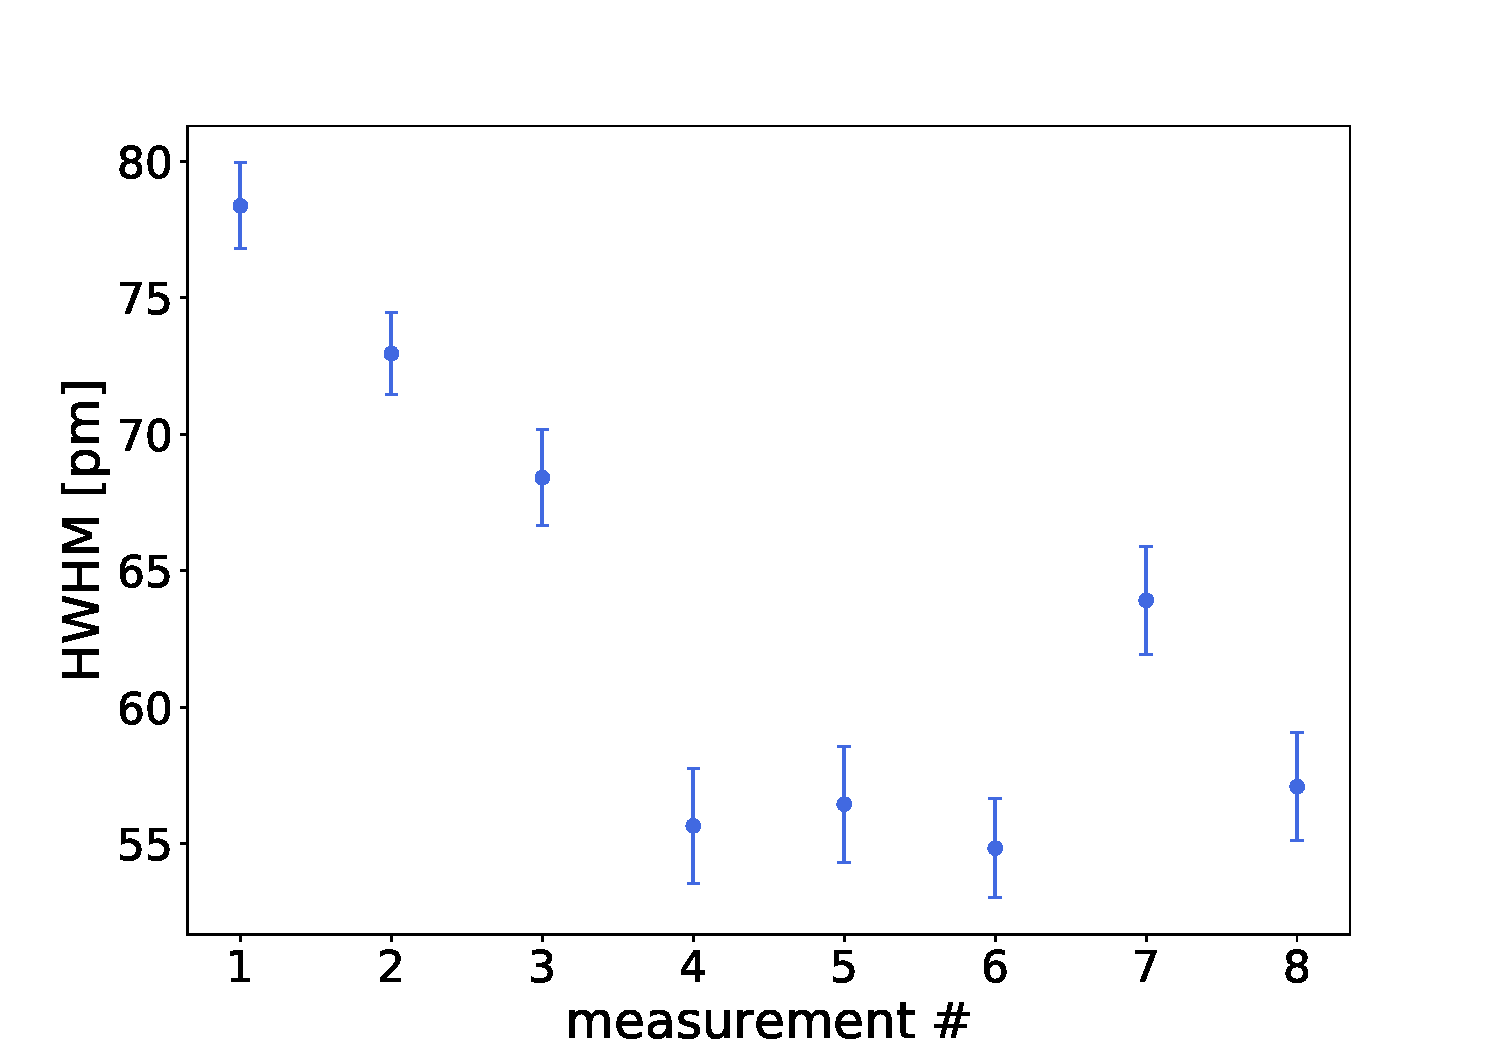
\includegraphics[width=0.7\textwidth]{figures/HWHM_vs_time_20250266_452um.pdf}
    \caption{Linewidth as a function of "time" of an approximately $452 \mu m$ double Fano cavity. It is clear that the linewidth generally decreases with time as a baseline for the HWHM is reached. This is assumed to be due to the drift of the piezo ring, while it must be noted that this is not possible to concluded indefinitely from the presented data. "Time" is to be understood as the chronological order in time, as the measurements are presented in the order in which they were recorded in the lab.}
    \label{fig:HWHM_vs_time}
\end{figure}

When the fringes of the time-dependent signal have been optimized fully, the frequency generator is then turned off and the fringes disappear. The piezo driver is now used to manually apply a constant voltage to expand the piezo gradually until the signal through the Fano cavity is maximized. This corresponds to the point where the cavity length and thus the cavity mode is resonant with the guided-modes of $G_1$ and $G_2$.

The piezo ring, while capable of tuning the cavity length on a very small scale, tends to drift with time. This drift is apparent when the constant voltage is applied as the signal tends to decrease with time after optimization of the transmission. The piezo drift is more pronounced when the measurement session is first started and the time it takes for the piezo to lengthen or shorten becomes longer when a constant voltage have been applied to the piezo for some time. For this reason the measurements of the Fano resonance transmission profiles tend to be broader at first, and then gradually converge to the optimal value as more measurements are conducted. Note however, that this varies greatly depending on the adjustments made throughout a measurement session. Figure \ref{fig:HWHM_vs_time} shows linewidths of the resonance transmission profile, of an arbitrarily chosen double Fano cavity, as a function of "time". "Time" is refering to the fact that the measurements are plotted in chronological order with respect to the time of measurement. 

\subsubsection{Determining the cavity length}

Now the double Fano cavity is aligned and the cavity-, laser- and guided-modes all coincide to a high enough degree to sustain a Fano resonance mode. However, before doing the actual optical charaterization, the cavity length must first be determined. In the end we want to plot the linewidth of the double Fano resonance spectra as a function of the cavity length, and in order to do so we must measure both. 

Here we remember that the Fano cavity, when off-resonance, acts simply as a Fabry-Perot intereferometer, which means that the off-resonance spectrum abides by the relations outlined in section \ref{sec:fabry_perot}. More specifically we know that the FSR relates to the cavity length according to eq. (\ref{eq:FSR_formula}), which can be re-interpreted, and re-written, as
\begin{equation}
    l = \frac{\lambda_0^2}{2 FSR},
\end{equation}
where $\lambda_0$ is the cavity resonance wavelength. 

So, to have a qualitative measure of the cavity length while doing measurements in the lab, off-resonance spectra are recorded and by estimating the FSR from the live data the approximate cavity length is determined.  

In order to obtain precise information on the length of a given cavity, we conduct more precise data analysis on the recorded off-resonance spectra. Figure \ref{fig:length_from_long_scan_example} shows two examples of off-resonance spectra for two cavities of different length. The lengths are found as a fitting parameters from a least squares fit of the recorded data to the Fabry-Perot transmission function found in eq. (\ref{eq:fabry_perot_trans}). 

\begin{figure}[h!]
    \centering
    \begin{subfigure}[b]{0.49\textwidth}
        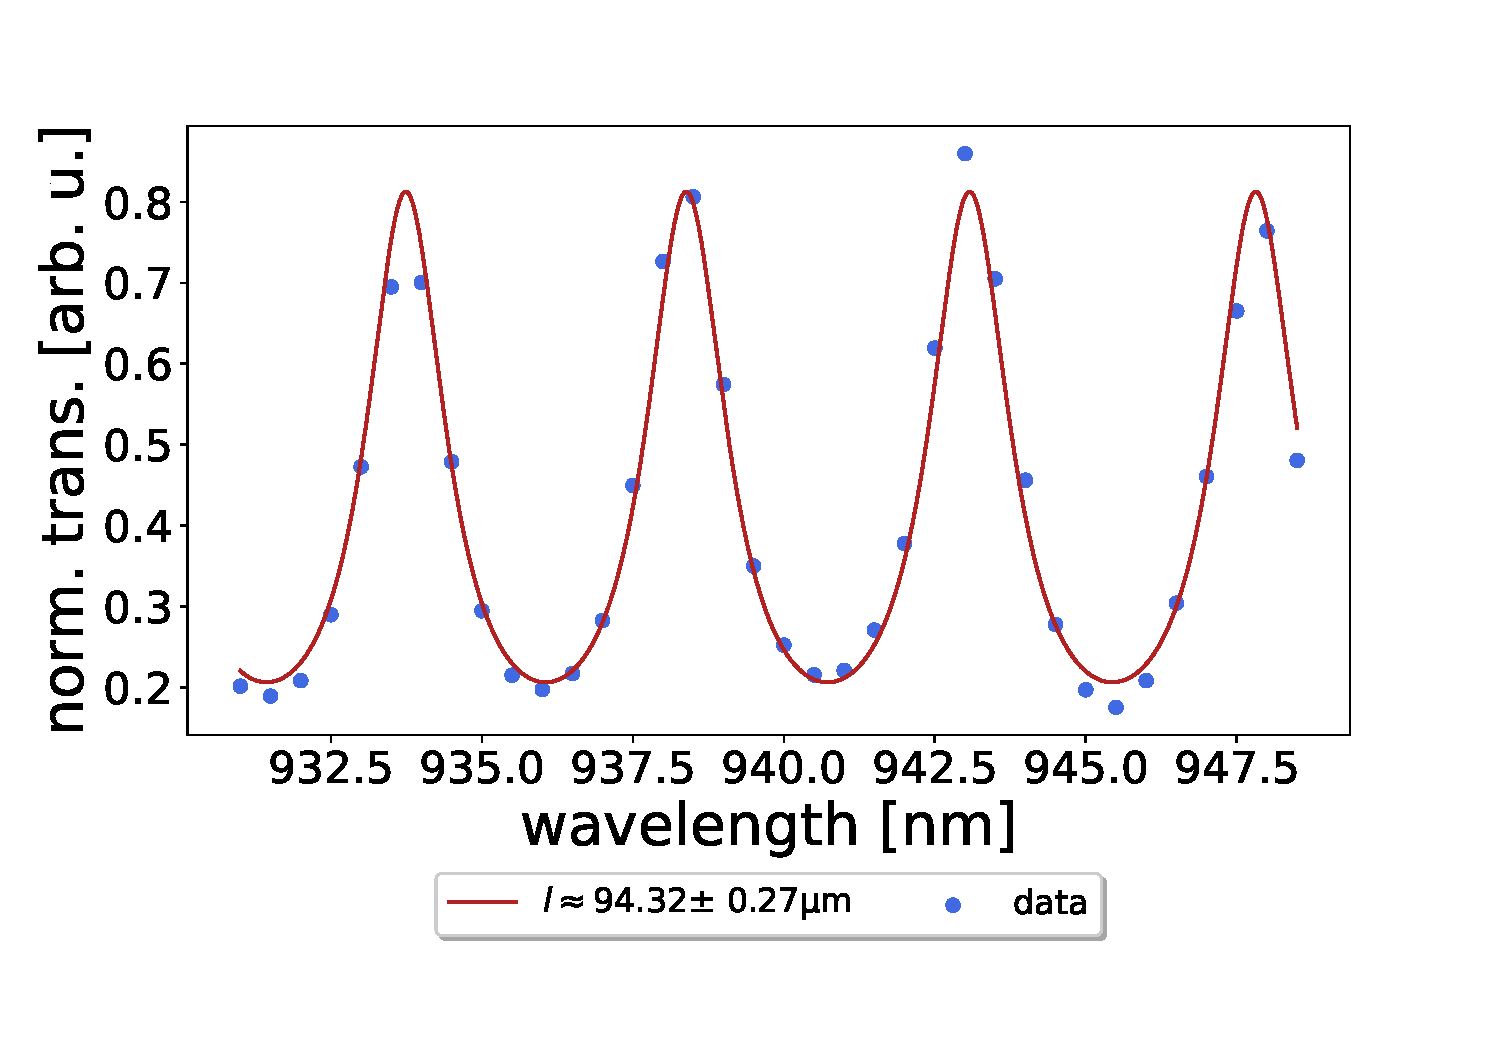
\includegraphics[width=\textwidth]{figures/length_from_fsr_example_100um.pdf}
        \caption{}
        \label{fig:100um_FSR}
    \end{subfigure}
    \begin{subfigure}[b]{0.49\textwidth}
        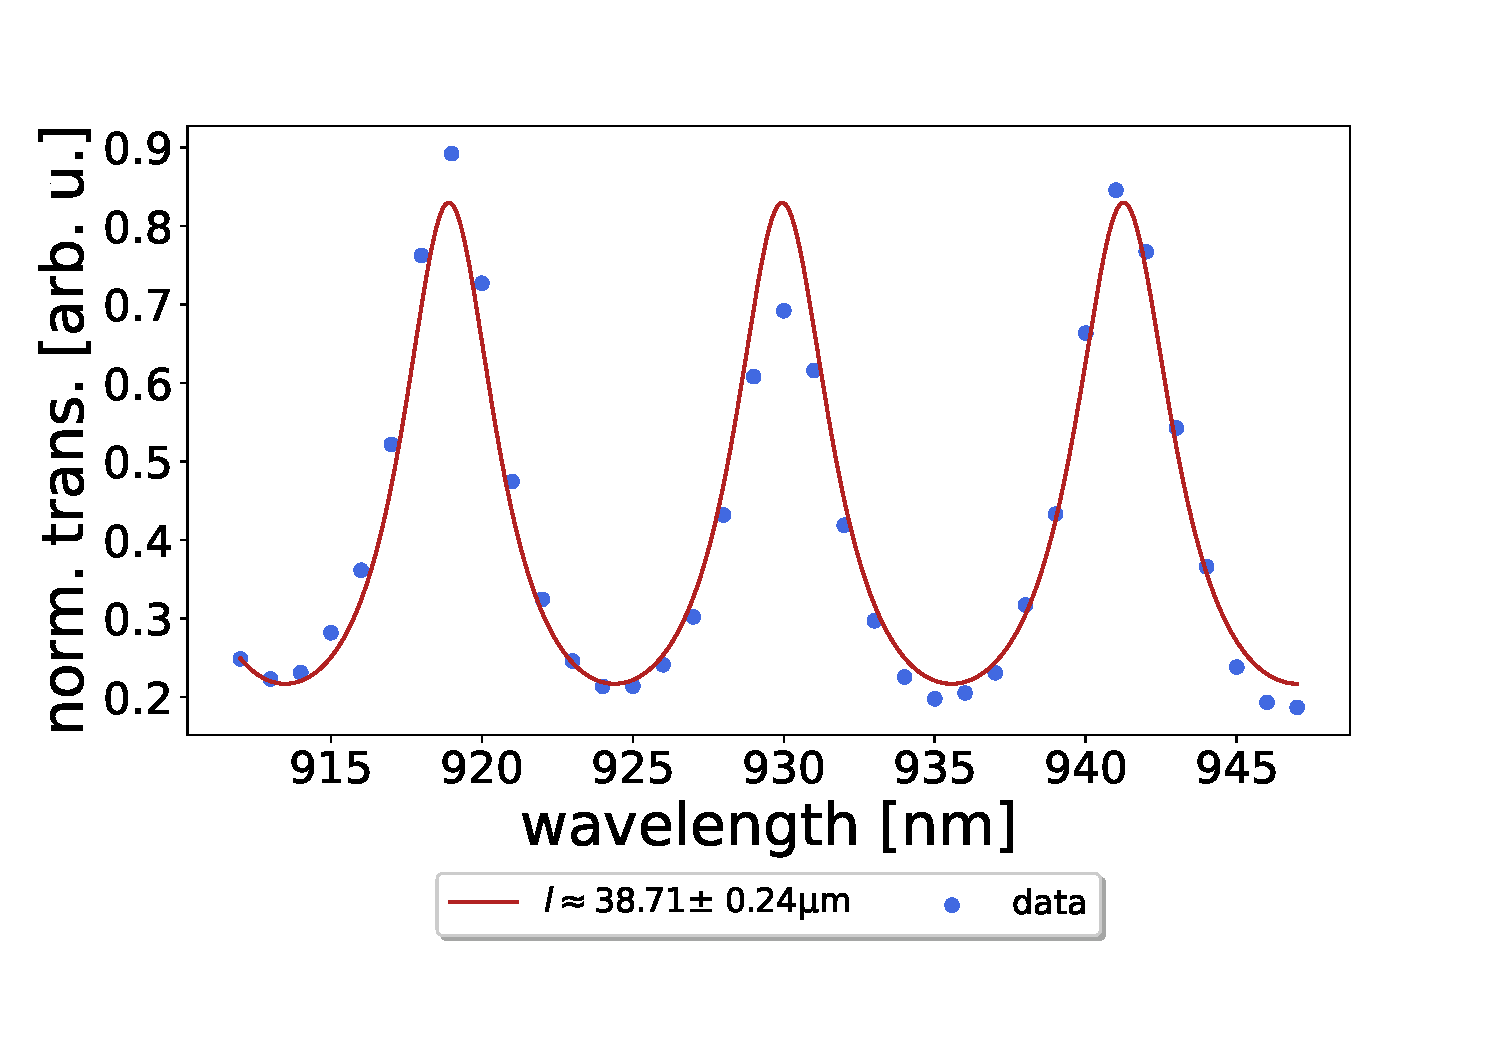
\includegraphics[width=\textwidth]{figures/length_from_fsr_example_40um.pdf}
        \caption{}
        \label{fig:40um_FSR}
    \end{subfigure}
    \caption{Off-resonance spectra of double Fano cavities of lengths $94.32 \pm 0.27 \mu m$ (a) and $38.71 \pm 0.24 \mu m$ (b). The lengths are found as fitting parameters from a least squarea fit of the recorded data to the Fabry-Perot transmission function in eq. (\ref{eq:fabry_perot_trans}), and the errors presented are found as the square root of the diagonal of the covarians matrix corresponding to the fit \cite{Hughes}. Note that the FSR increases when the cavity length decreases, as predicted in eq. (\ref{eq:FSR_formula}).}
    \label{fig:length_from_long_scan_example}    
\end{figure}


\subsubsection{Recording normalized spectra}

The normalized spectra are now recorded in largely the same way as for the individual Fano mirrors in section \ref{sec:grating_characterization}, a series of measurements is necessary in order to obtain meaningful spectra that are normalized with respect to the light incident on the cavity. The needed measurements are the following: 
\begin{enumerate}
    \item The transmission through the Fano cavity recorded in photo detector $P_T$ where the corresponding values for the measured amplitudes are denoted $T$.
    \item The light recorded in photo detector $P_I$ during the transmission measurement. The corresponding values for the measured amplitudes are denoted $T_I$.
    \item The light recorded in photo detector $P_T$ when no cavity is present in the setup. This is denoted $P_T^{\prime}$. The corresponding values for the measured amplitudes are denoted $T^{\prime}$.
    \item The light recorded in detector $P_I$ during the transmission measurement with no cavity present. This is similarly denoted $P_I^{\prime}$. The corresponding values for the measured amplitudes are denoted $T_I^{\prime}$.
\end{enumerate}

\begin{figure}[h!]
    \centering
    \begin{subfigure}[b]{0.49\textwidth}
        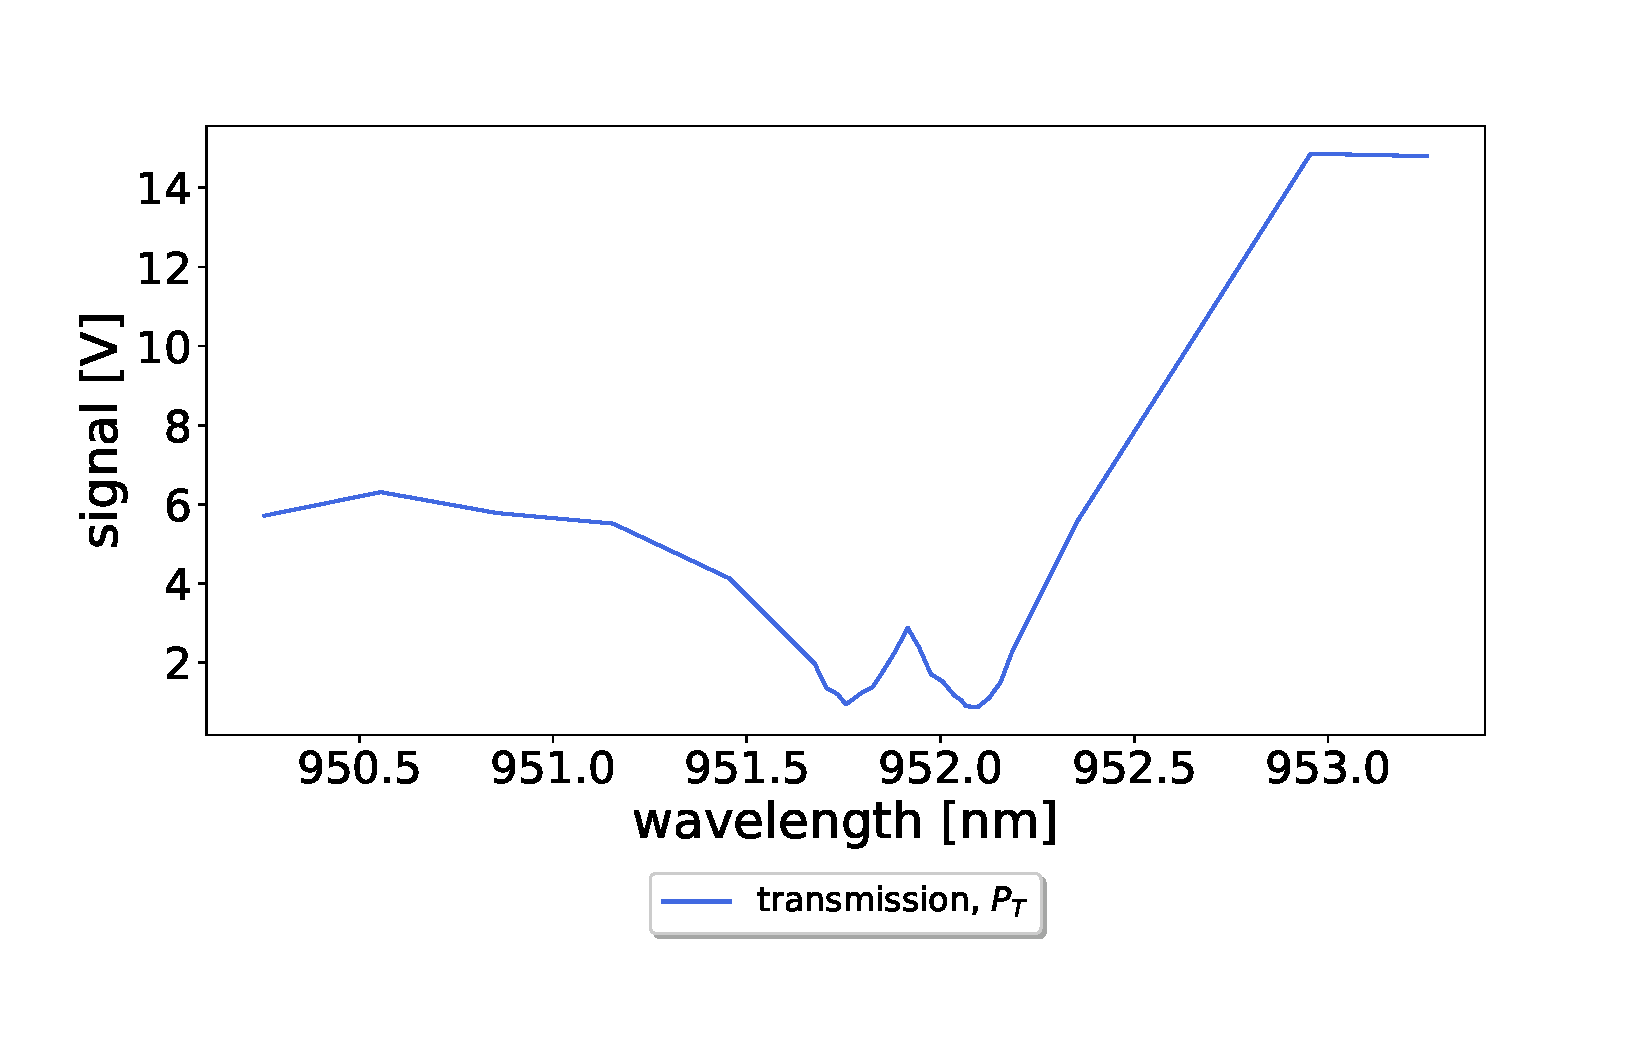
\includegraphics[width=\textwidth]{figures/raw_data_cavity_trans.pdf}
        \caption{}
        \label{fig:raw_data_trans_with_cavity}
    \end{subfigure}
    \begin{subfigure}[b]{0.49\textwidth}
        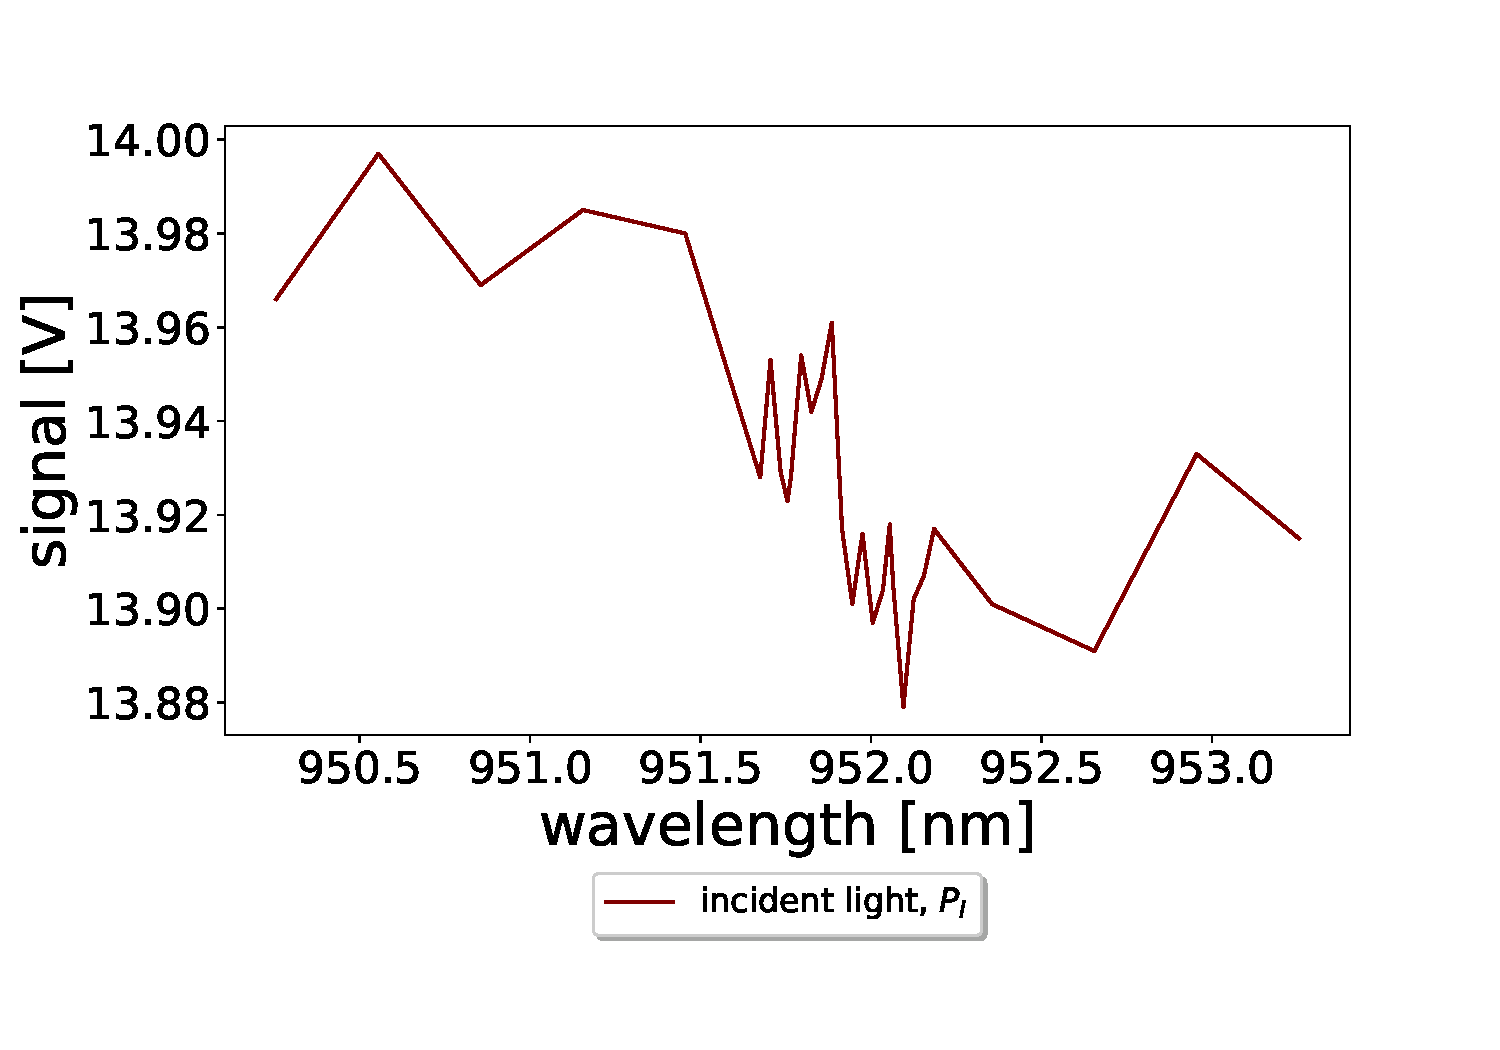
\includegraphics[width=\textwidth]{figures/raw_data_incident_light_cavity.pdf}
        \caption{}
        \label{fig:raw_data_incident_with_cavity}
    \end{subfigure}
    \begin{subfigure}[b]{0.49\textwidth}
        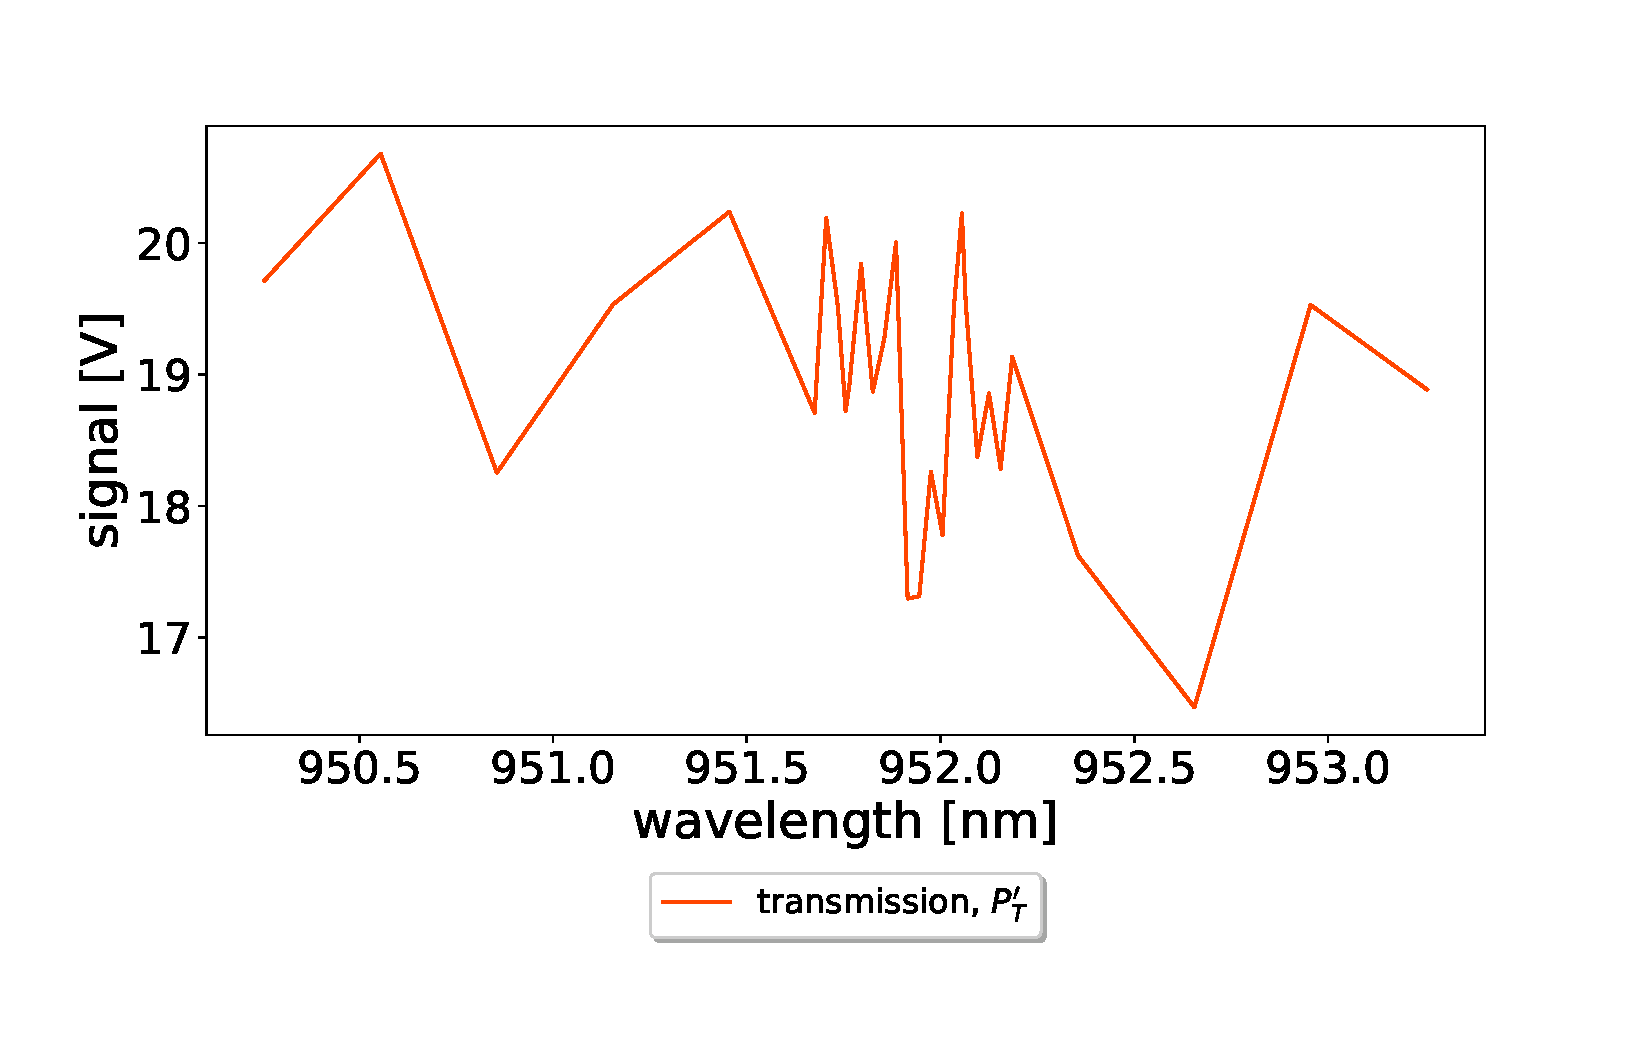
\includegraphics[width=\textwidth]{figures/raw_data_transmission_no_cavity.pdf}
        \caption{}
        \label{fig:raw_data_trans_no_cavity}
    \end{subfigure}
    \begin{subfigure}[b]{0.49\textwidth}
        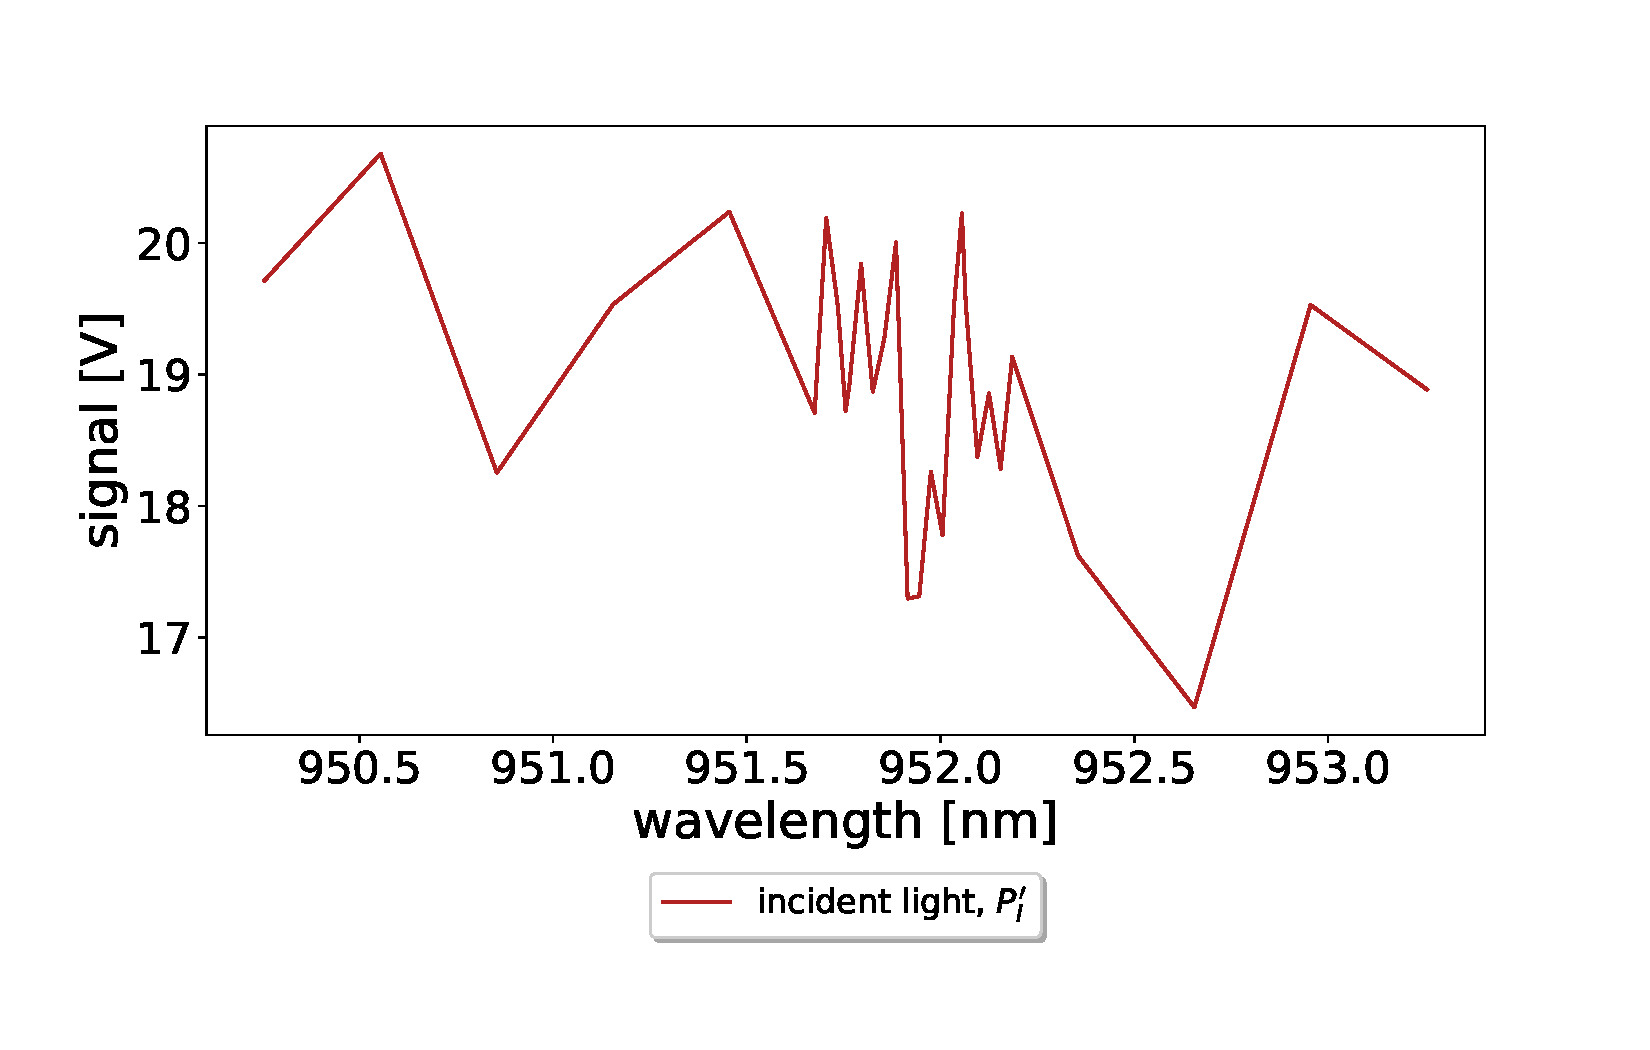
\includegraphics[width=\textwidth]{figures/raw_data_incident_light_no_cavity.pdf}
        \caption{}
        \label{fig:raw_data_incident_no_cavity}
    \end{subfigure}
    \caption{Examples of the four measurements used to produce the normalized transmission spectrum of the double Fano cavity (the same naturally applies for the single Fano cavity transmission). (a) shows the transmission through the double Fano cavity, (b) shows the incident light on the cavity, (c) shows the "transmission" when no cavity is present and (d) shows the light recorded by the incidence detector with no cavity present. All data is recorded for the same cavity of length $l=21.390 \pm 0.119 \mu m$. Note that the spectra in (c) and (d) seem identical. This is to be exprected as they are simply measurements of a beam in each arm of a $50/50$ beam splitter.}
    \label{fig:raw_data}
\end{figure}

The normalized transmission values are then given as
\begin{equation}
    T_{norm} = \frac{T/T_I}{T^{\prime}/T_I^{\prime}},
    \label{eq:normalized_cavity_spectrum}
\end{equation}
which is the exact formula used for the Fano mirror characterization, except for the subtraction of the background which has here been assumed negligible. Examples of the four measurements are seen in figure \ref{fig:raw_data}, and the normalized spectrum is correspondingly seen in figure \ref{fig:raw_data_normalized_transmission}.

\begin{figure}[h!]
    \centering
    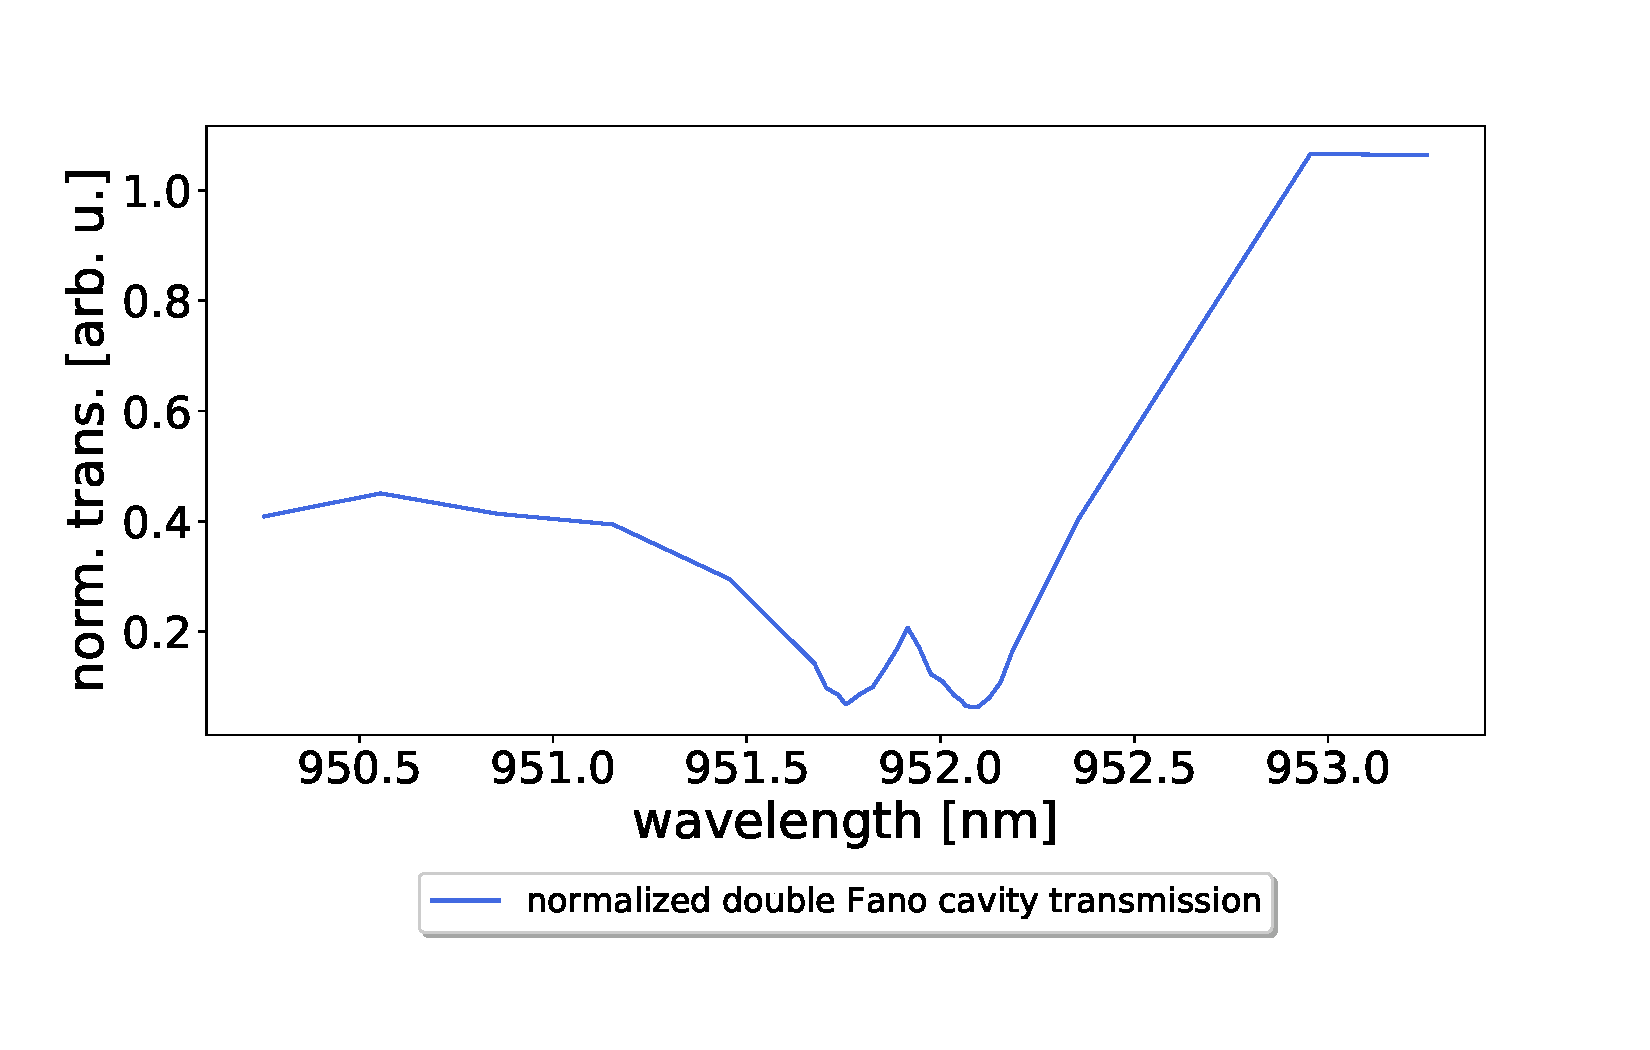
\includegraphics[width=0.7\textwidth]{figures/raw_data_normalized_transmission.pdf}
    \caption{The normalized transmission spectrum for a double Fano cavity of length $l=21.390 \pm 0.119 \mu m$ calculated from the data depicted in figures \ref{fig:raw_data}a-d using eq. (\ref{eq:normalized_cavity_spectrum}).}
    \label{fig:raw_data_normalized_transmission}
\end{figure}

\subsubsection{Centering of the top grating}\label{sec:pinhole_method}

When aligning the top part of the cavity setup seen in figure \ref{fig:setup_top_sketch_and_pic}, it is crucial to ensure that the beam passes through the center of the rotational mount. Even the slightest deviation from the center can cause the alignment to be tedious at best, but likely practially impossible. The reason for this is the need for invariance in the xy-plane when aligning the Fano mirror for the fixed polarization of the laser. If the deviation from the center is too large, it might be impossible to tell whether the change in the transmitted intensity stems from moving further or closer to the optimal polarization, or if the Fano mirror is simply moving in and out of the beam. For this alignment a pinhole was designed to fit with high precision into the rotational mount in which it was fastened with a one inch (\emph{SM1}) retainer ring from Thorlabs. A simple sketch of the pinhole is seen in figure \ref{fig:pinhole_sketch}.

\begin{figure}[h!]
    \centering
    \begin{subfigure}[b]{0.49\textwidth}
        \centering
        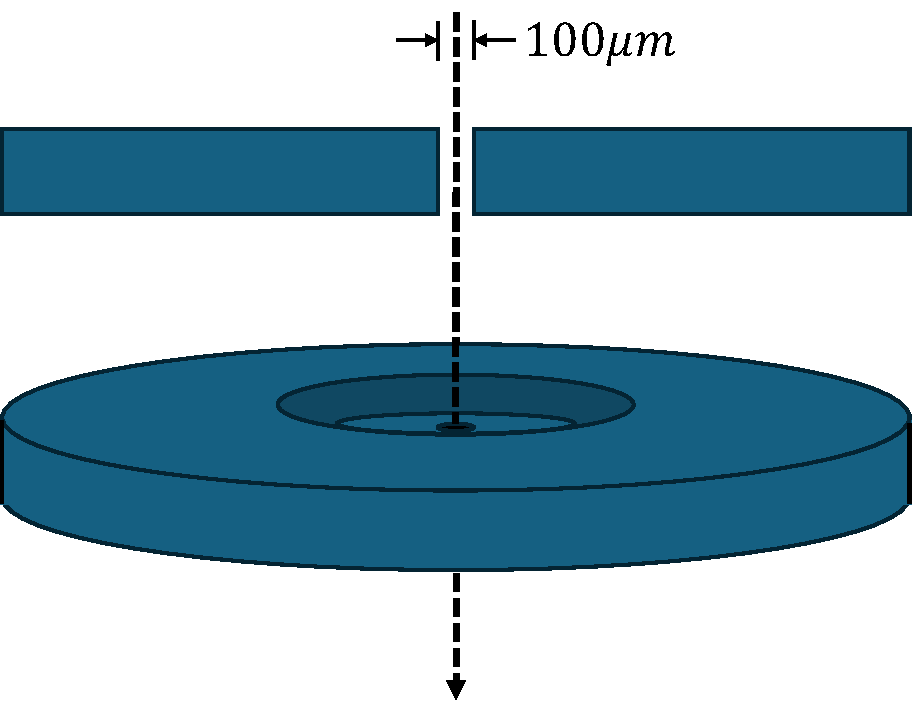
\includegraphics[height=6cm]{figures/pinhole_sketch.pdf}
        \caption{}
        \label{fig:pinhole_sketch}
    \end{subfigure}
    \hfill
    \begin{subfigure}[b]{0.49\textwidth}
        \centering
        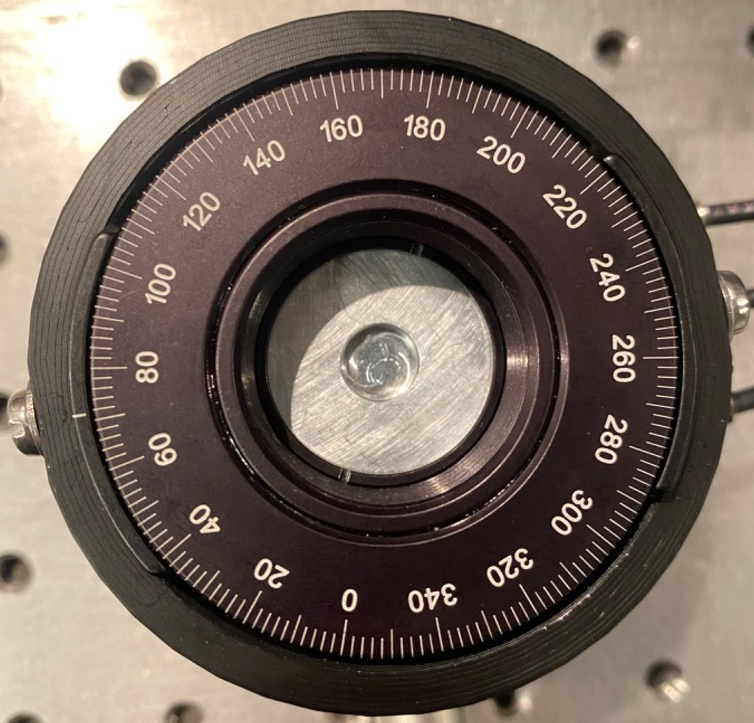
\includegraphics[height=6cm]{figures/pinhole_picture.pdf}
        \caption{}
        \label{fig:pinhole_picture}
    \end{subfigure}
    \caption{In (a) is a sketch of the pinhole used for centering the rotational- and kinetic mirror mounts in the incident beam. The side view of the pinhole is included to mark the pinhole diameter clearly while the angled view provides a visual representation of the actual component. (b) shows a picture of the rotational mount, seen from the top, with the pinhole inserted.}
    \label{fig:pinhole_sketch_and_picture}
\end{figure}

By moving the xy-stages in the cavity setup, it proved possible to achieve the centering of the rotational mount by moving the setup, with the pinhole inserted, until the transmission signal was maximized. Another test of the alignment was here to rotate the mount and thus pinhole and ensure that the signal intensity was as close to rotationally invariant as possible. Figure \ref{fig:pinhole_position_on_gaussian} shows an arbitrary gaussian distribution resembling the transverse distribution of a laser beam in the TEM00 mode and two shaded regions imitating the position of the pinhole. The red shaded region shows an \emph{unaligned} pinhole position while the green one is perfectly \emph{aligned} in the center of the beam. It is shown on the figure that the red area covers an intensity corresponding to $15.8\%$ of the maximum intensity, while this value for the aligned green region is approximately double at $30.53\%$.

\begin{figure}[h!]
    \centering
    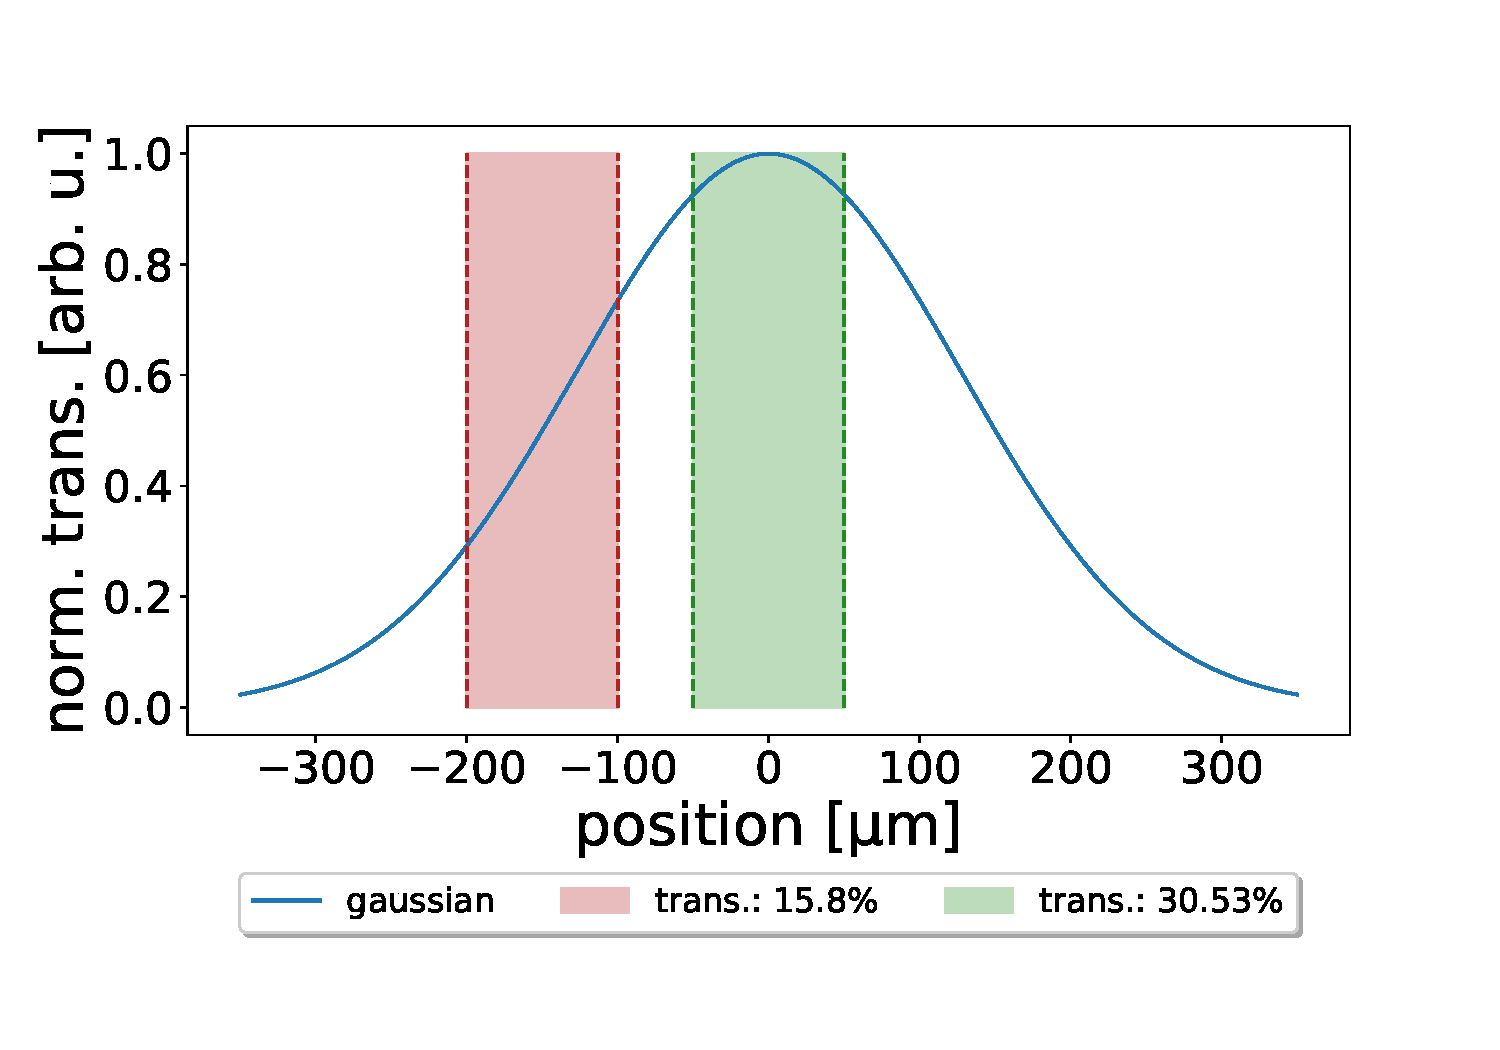
\includegraphics[width=0.7\textwidth]{figures/pinhole_position_on_gaussian.pdf}
    \caption{A gaussian distribution corresponding to the transverse distribution of a laser in the TEM00 mode. The red shaded region indicates a position for the pinhole with a transmission of $15.8\%$ while the green one indicates a position with a transmission of $30.53\%$. The spacial dependence of the transmission through the pinhole is thus clearly displayed.}
    \label{fig:pinhole_position_on_gaussian}
\end{figure}

\subsubsection{Estimating parallelism}\label{sec:parallelism}

A key difference between the single and double Fano cavity transmission spectra, is the off-resonance behavior. While the maximum transmission intensity for the single Fano will generally be lower than the Fano resonance peak, the opposite tends to be the case for the double Fano cavity. The direct reflectivities and transmissions $r_d$ and $t_d$ are similar, if not identical, for the two Fano mirrors, which means that the off-resonance Fabry-Perot-like transmission reaches a maximum of close to unity. The initial alignment of the cavity can thus be done by maximizing the off-resonance fringes. Due to the much broader peaks in this spectral regime, the fringes will be much less sensitive than the resonance peak. For this reason additional optimization is likely necessary. 

Nair et al. \cite{Nair} has proposed an analytical formula to estimate the wedge angle by considering the maximum transmission $T_{MAX}$ of these Fabry-Perot fringes. $T_{MAX}$ is given as 
\begin{equation}
    T_{MAX} \approx 1 - \left(\frac{F \pi w_0}{\lambda}\right)^2 \varepsilon^2,
\end{equation}
for a cavity of identical resonators, and as this is not necesarrily the case for an arbitrary double Fano cavity we make the substitution $1 \rightarrow T_{MAX}^{optimal}$ to include the highest possible transmission given a set of compatible Fano mirrors. The expression now simply reads
\begin{equation}
    T_{MAX} \approx T_{MAX}^{optimal} - \left(\frac{F \pi w_0}{\lambda}\right)^2 \varepsilon^2,
\end{equation}
where $T_{MAX}^{optimal}$ is the maximum transmission for a wedge angle of $0$, $w_0$ is the beam waist, $\lambda$ is the wavelength, $\varepsilon$ is the wedge angle in radians and $F$ is the coefficient of finesse \cite{Pedrotti} given as
\begin{equation}
    F = \frac{4R}{(1-R)^2}.
\end{equation}
Rearranging this, for the wedge angle $\varepsilon$ we get
\begin{equation}
    \varepsilon \approx \sqrt{\left(T_{MAX}^{optimal} - T_{MAX} \right)} \left(\frac{\lambda}{F \pi w_0}\right).
\end{equation}
An example of a normalized off-resonance transmission spectrum of a double Fano cavity is shown in figure \ref{fig:parallelism_plot}. The blue line indicates a least squares fit of the data points to the Fabry-Perot transmission function seen in eq. (\ref{eq:fabry_perot_trans}), while the red line indicates the optimal transmission for the same Fano mirrors as was used for the measurement. The maximum transmission recorded and the optimal value was found as
\begin{equation}
    T_{MAX} = 83.3\% \hspace{0.5cm} \text{and} \hspace{0.5cm} T_{MAX}^{optimal} = 97.1\%,
\end{equation}
which yields for the wedge angle 
\begin{equation}
    \varepsilon \approx 0.24 \: \text{mrad} = 0.014^{\circ},
\end{equation}
assuming a beam waist of $w_0 = 160 \mu m$ and direct refletivities and transmissions $r_d = 57\%$, $r_d^{\prime} = 57.5\%$ and $t_d = t_d^{\prime} = 81.4\%$.

\begin{figure}[h!]
    \centering
    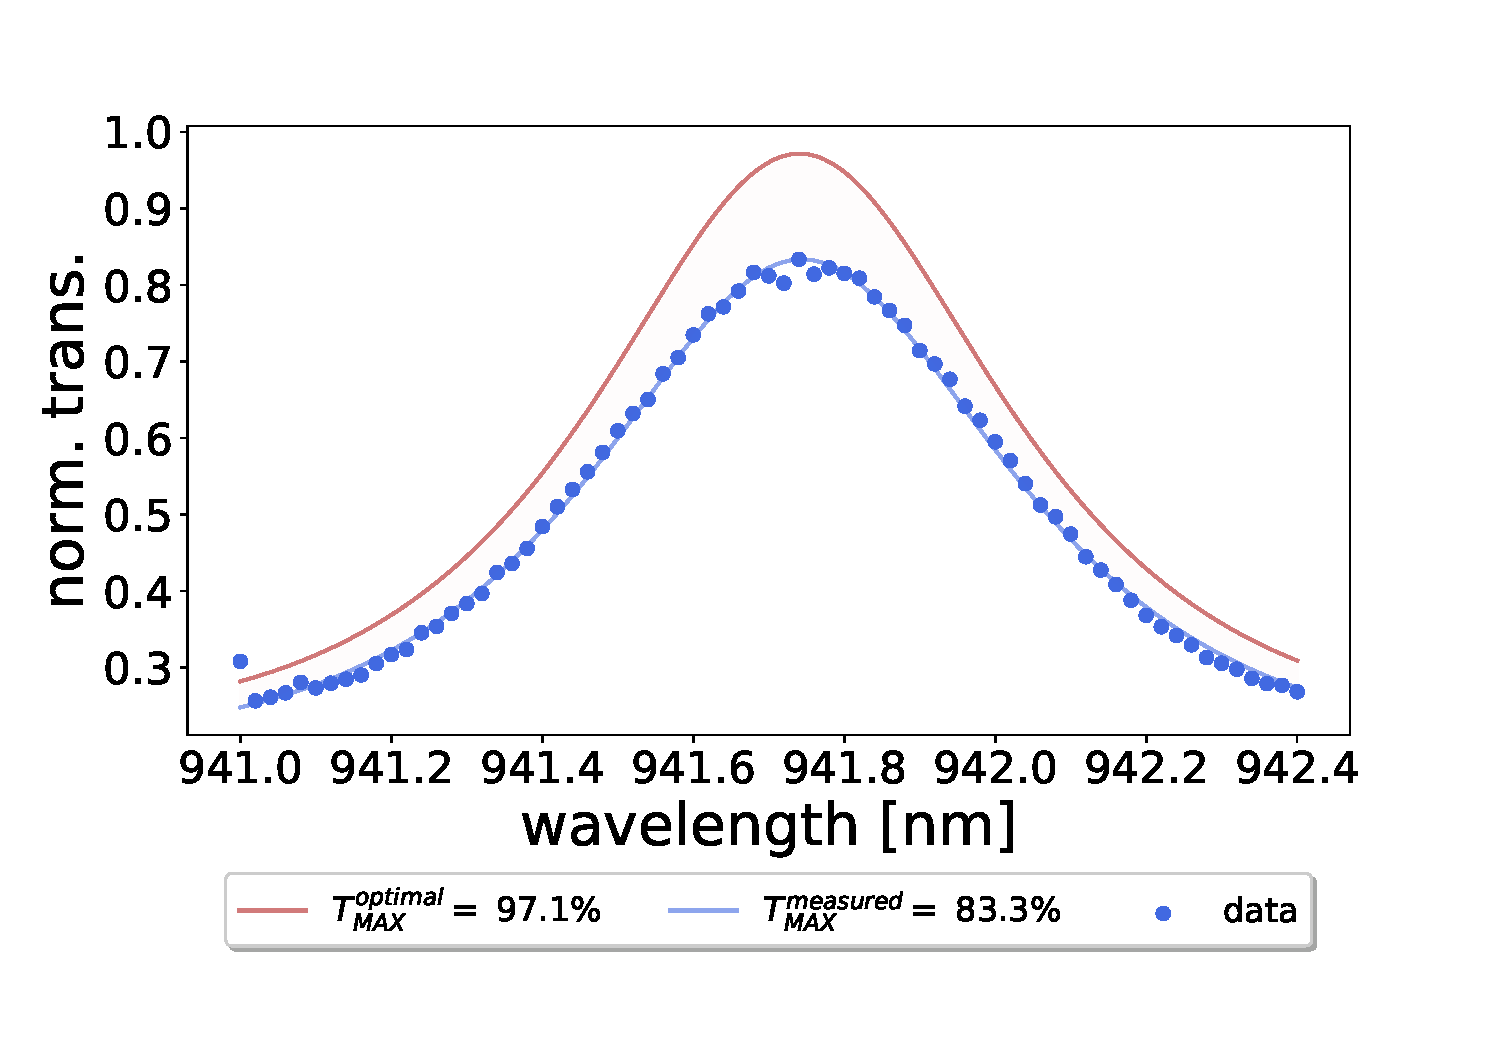
\includegraphics[width=0.7\textwidth]{figures/parallelism_plot.pdf}
    \caption{Example of a normalized off-resonance transmission peak of a double Fano cavity of direct reflectivities $r_d = 57\%$ and $r_d^{\prime}=57.5\%$ and direct transmissions $t_d = t_d^{\prime} = 81.4\%$. The blue line is a least squares fit of the data to the Fabry-Perot transmission function while the red line is the optimal value of the same function. The red shaded area indicate the differnce between the two.}
    \label{fig:parallelism_plot}
\end{figure}

It is thus clear that while the sensitivity is of the off-resonance Fabry-Perot fringes is lower than that of the Fano resonance peak, they still provide a significant measure of the parallelism and is thus useful for initial cavity alignment.
